\chapter{Ardupilot} \label{ch:4}
\textcolor{red}{Flow diagram Angus showen.}

The software on which the drone runs on is called Ardupilot. Ardupilot is an open source available software, which is developed by a team of diverse professional engineers and computer scientists [2] \url{http://ardupilot.org/about}. The software is capable of controlling multirotors and other vehicles, which is easy adjustable to desire. Figure \ref{fig:ardupilotbase} shows a highlevel view of the ardupilot architecture.

\begin{figure}[H]
\centering
\includegraphics[width=\textwidth]{ardupilotbase.PNG}
\caption{Highlevel view of the ardupilot architecture.}
\label{fig:ardupilotbase}
\end{figure}

Zooming a bit closer explains the code better. As can be seen in Figure \ref{fig:ardupilotbasezoom}, the base of the code is divided in several subfunctions which are explained in this chapter.

\begin{figure}[H]
\centering
\includegraphics[width=\textwidth]{ardupilotbasezoom.PNG}
\caption{Zoomed highlevel view of the ardupilot architecture.}
\label{fig:ardupilotbasezoom}
\end{figure}

\section{Main loop}

The software runs with a main loop working at a 400 Hz frequency.

\section{Flight mode}
Flight mode checks the vehicle's flight mode and calls the matching function. A flight mode converts the given input by the user into a lean angle, climb rate, etc. that is suitable for that flight mode. A few flightmodes, which are used throughout the project, are explained in detail.
\begin{itemize}
\item Stabilize: This modes allows manual flying, with automatic control of the roll and pitch axis. The automated roll and pitch control ensures the drone from not tilting, however it can experience drift by wind. The pilot can counter this by giving a lean angle input to the copter. With respect to yaw, the pilot can give a yaw-rate input to apply yaw rotations. Furthermore does the pilot has to give enough thrust input so that the drone maintains altitude. Give less thrust to descent and give more to climb.\\

\item Loiter: automatically attempts to maintain the current location, heading and altitude. When no lean angle input is given by the pilot, the vehicle will try to hold position. Furthermore can the pilot give lean angles input to move in horizontal plane and can the altitude be altered by increasing or decreasing throttle input. Thereby it is needed to have good GPS connection, low magnetic interference on the compass and low vibrations to achieve good loiter performance.\\

\item AltHold: The copter maintains altitude while allowing roll, pitch and yaw to be controlled normally. This means that the throttle will be automatically controlled to maintain altitude. Operating in lean angles will be the same as in Stabilize mode.\\

\item Auto: This mode is a combination of different modes, since it uses altitude control from AltHold and the position control from Loiter. Auto mode is able to fly a pre-programmed mission, which will take the drone from given location to location. After taken the desired path, a Return To Launch can be used to land at Home, which is the initiated location where the vehicle was armed.\\
\end{itemize}

\section{Position Control}




\section{Attitude control}
The attitude control defines the controller to convert the Roll/Pitch/Yaw errors (the difference between the target angle and actual angle) into the desired rotation rate followed by a PID controller to vonvert the rotate rate error into a high level motor command. A flow scheme has is visible in Figure \ref{fig:attitudecontrol}.

\begin{figure}[H]
\centering
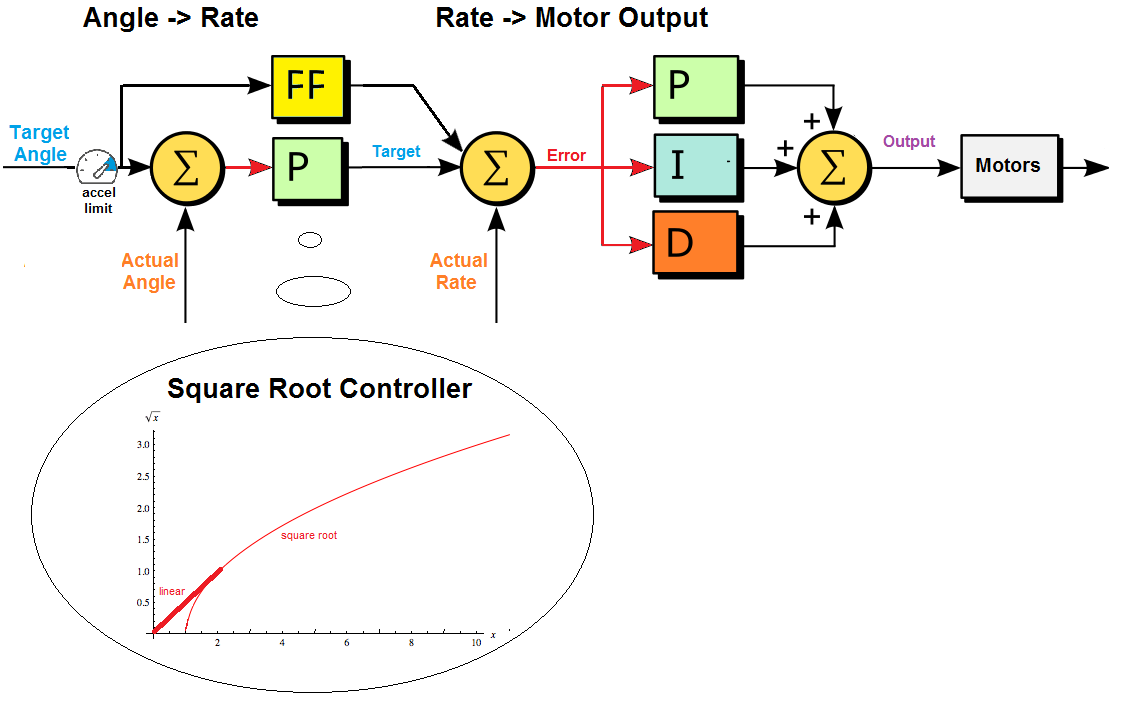
\includegraphics[width=\textwidth]{Attitudecontrol.PNG}
\caption{Flow diagram showing the attitude control per axis.}
\label{fig:attitudecontrol}
\end{figure}

$AC_AttitudeControl$ library

\section{Motor and Servo Control} 


\section{Other}
Furthermore are there some other functions which can be added to Ardupilot as well, i.e. other sensor drivers.\\
Frame orientation. \\
Motor mixing.\\

